\chapter{Experimental Setup}
\label{cha:procedure}

\section{The Coal Chamber}

  The experiments is carried out under UHV (ultra high vacuum) conditions. This is crucial because contaminants easily can absorb to the surface which ruins the quality of the gathered data. During this project the vacuum chamber named 'The Coal Chamber' is used which is one of many vacuum chambers in the SDL lab.\\
  The equipment mounted on The Coal Chamber, which is used in this study, is described in the following section along with the experimental approach. The sample is introduced to the coal chamber from a loadlock where the sample is attached to a transfer arm. Transfer of the sample from the loadlock to the main chamber takes place as the pressure in the loadlock is reduced sufficiently by a turbo pump. In the main chamber a manipulator is apparent in the center from where the sample can be transferred to the STM by a wobble stick. A filament lies behind the sample in the manipulator, which is used during anneals.

\subsection{Turbo pump}

  In order to achieve proper UHV conditions a turbo pump is needed in addition to the roughing pump. The turbo pump is directly connected to the vacuum chamber and consists of a series of rotor blades. Each of these adds momentum to the remaining gas molecules that collide with the blades and hence removes these from the chamber. In order to function properly these rotor blades spins up to 80.000 RPM.\cite{hofTurbo}

\subsection{H2 cracker - Vibrationally excited molecules}

Vibrationally excited molecules are produced using a H$_2$ cracker.

\section{STM}

The STM was used to get a visualization of the coverage of hydrogen on the sample surface, and to analyse the sample between the different experiments.


write things about linescans, calibration and FFT/noise removal.

\section{TPD}

A mass spec is connected to the UHV chamber, and this was used to investigate the desorption of deuterium from the sample surface. The sample was positioned in the manipulator as the experiments were carried out. From here the nozzle of the mass spec was brought within millimeters of the sample. The temperature was logged together with the amount of deuterium detected by the mass spec. The mass spec was set to count masses of 4 amu, in order to exclude other molecules than deuterium. This setup was made with the computer program 'MASsoft' by Hiden Analytical.\\
A Eurotherm 2704 controller was used to control the current going to the filament in the manipulator, in order to manage the temperature of the sample. The controller was programmed to ramp the sample temperature from 300K to 900K at a rate of 1K per second. At maximum temperature the eurotherm was set to rest for 30s, and then slowly decrease the temperature to a final temperature of 300K. This cycle was performed each time a TPD measurement was carried out. During this procedure most of the deuterium on the surface should be desorped from the sample.\\
\begin{align*}
  T_{surface} = T_{TC} * 0.7921 + 131.2
\end{align*}
\begin{figure}
  \centering
  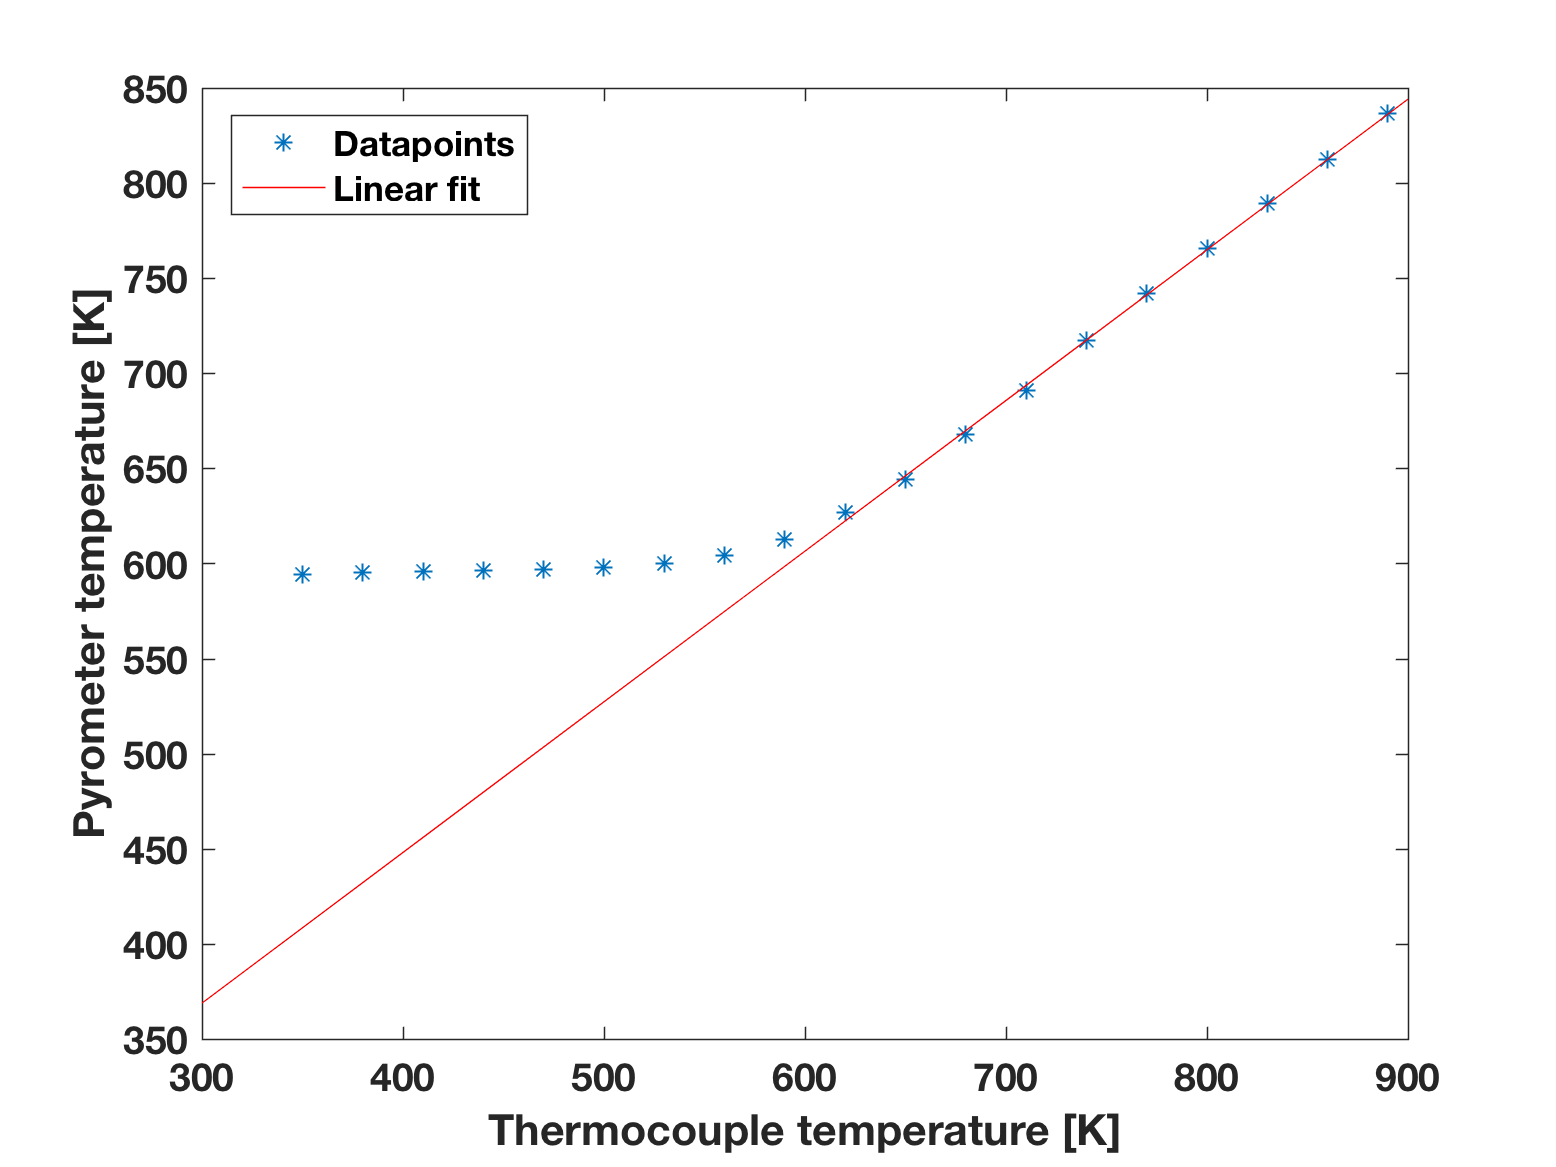
\includegraphics[width=0.55\textwidth]{TPD/kalibrering}
  \caption{Calibration of the temperature during the TPD measurements. The temperature of the surface measured by an optical pyrometer is plotted against the thermocouple temperature.}
  \label{TPDcalibration}
\end{figure}
In figure \ref{TPD:example} the data obtained from a typical TPD measurement is shown. Since the desorption of deuterium from the surface is investigated, a mass of 4 amu is monitored along with the temperature. It is seen that the temperature follows the linear trend except for the extremities of the temperature interval where some fluctuations start to happen. Since the temperature is controlled and logged with the Eurotherm controller, it is possible to plot the counts of deuterium against the temperature. These plots are presented in chapter \ref{cha:results}.\\
A triple gaussian function was fitted to the datapoints around the peak, in order to determine the temperature belonging to the peak. The peak value was estimated by visual observation, and the datapoints within $\pm$60\degree C are included in the fit. The temperature at the maximum of the fit was determined, and these values are presented in chapter \ref{cha:results} as the peak temperatures. An example of the fit to the peak values is shown in figure \ref{TPD:peak}. From this figure it is seen that the temperature at which the maximum counts is observed, not necessarily corresponds to the correct peak temperature. The green circle in figure \ref{TPD:peak} shows the found peak from which the temperature was gathered.\\
In order to compare the individual peaks, the background was subtracted from every datapoint. The sample was positioned stationary in front of the nozzle for a period of time before the measurements were carried out. These datapoints were used to calculate a mean background count, which was subtracted.

\begin{figure}[H]
  \centering
  \begin{subfigure}[b]{0.45\textwidth}
    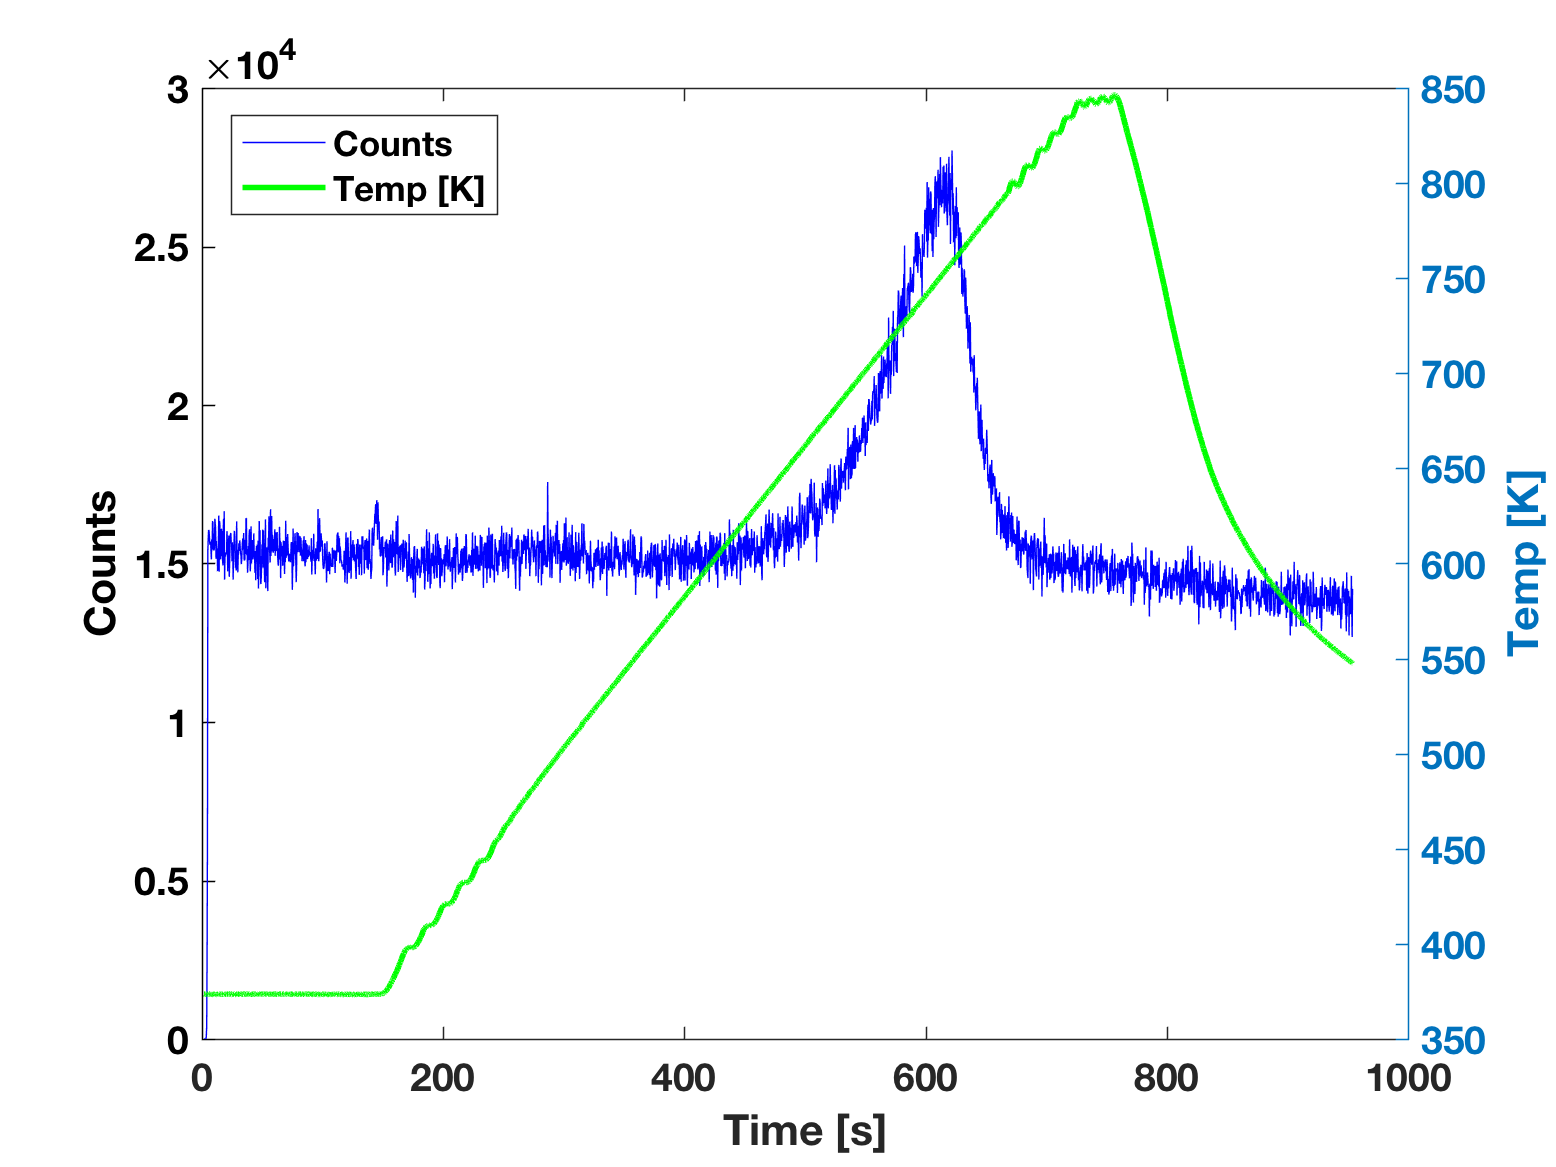
\includegraphics[width=\textwidth]{TPD/GrIr1740CD2_2504}
    \caption{}
    \label{TPD:example}
  \end{subfigure}
  \begin{subfigure}[b]{0.45\textwidth}
    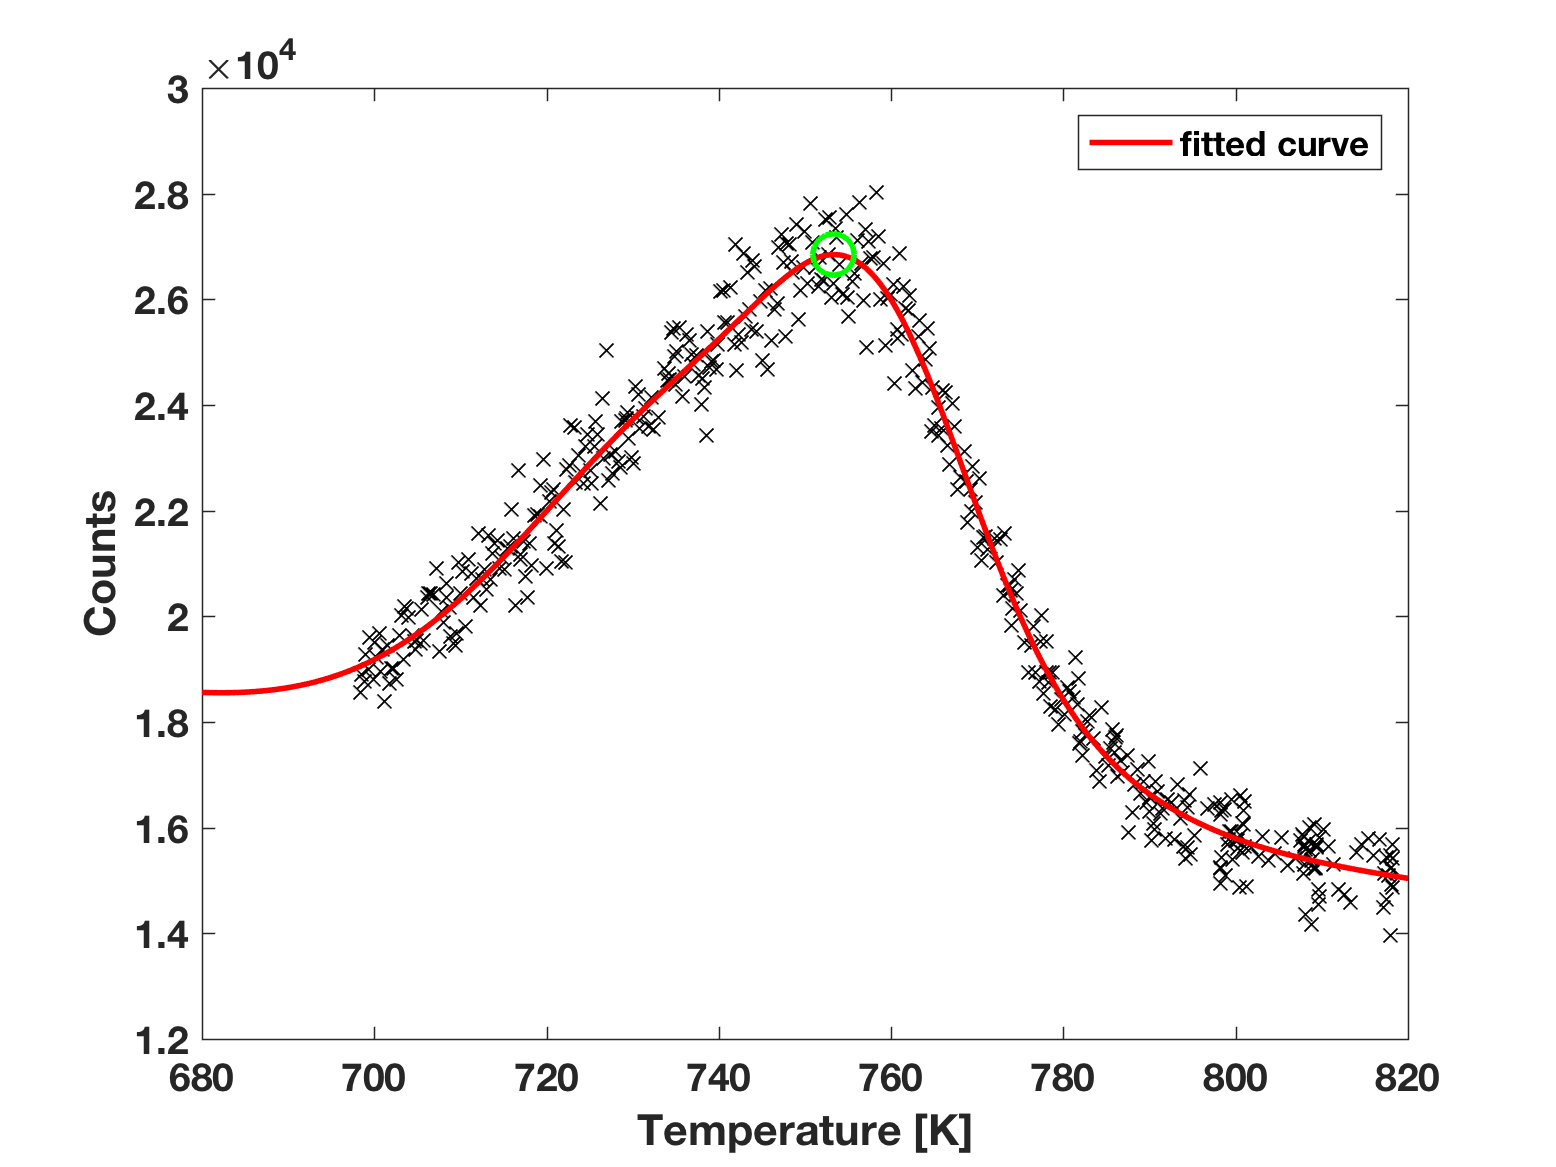
\includegraphics[width=\textwidth]{TPD/GrIr1740CD2_2504peak}
    \caption{}
    \label{TPD:peak}
  \end{subfigure}
\end{figure}
